%%%%%%%%%%%%%%%%%%%%%%%%%%%%%%%%%%%%%%%%%
% Programming/Coding Assignment
% LaTeX Template
%
% This template has been downloaded from:
% http://www.latextemplates.com
%
% Original author:
% Ted Pavlic (http://www.tedpavlic.com)
%
% Note:
% The \lipsum[#] commands throughout this template generate dummy text
% to fill the template out. These commands should all be removed when 
% writing assignment content.
%
% This template uses a Perl script as an example snippet of code, most other
% languages are also usable. Configure them in the "CODE INCLUSION 
% CONFIGURATION" section.
%
%Assignment 9
%Author Zetan
%%%%%%%%%%%%%%%%%%%%%%%%%%%%%%%%%%%%%%%%%

%----------------------------------------------------------------------------------------
%	PACKAGES AND OTHER DOCUMENT CONFIGURATIONS
%----------------------------------------------------------------------------------------

\documentclass{article}

\usepackage{fancyhdr} % Required for custom headers
\usepackage{lastpage} % Required to determine the last page for the footer
\usepackage{extramarks} % Required for headers and footers
\usepackage[usenames,dvipsnames]{color} % Required for custom colors
\usepackage{graphicx} % Required to insert images
\usepackage{listings} % Required for insertion of code
\usepackage{courier} % Required for the courier font
\usepackage{multirow}
\usepackage{listings,multicol}
\usepackage{pgfplots,pgfplotstable}
 \usepackage{amssymb}
 \usepackage{float}

\usepackage{url}
\usepackage{longtable}

% Margins
\topmargin=-0.45in
\evensidemargin=0in
\oddsidemargin=0in
\textwidth=6.5in
\textheight=9.0in
\headsep=0.25in

\linespread{1.1} % Line spacing

% Set up the header and footer
\pagestyle{fancy}
\lhead{\hmwkAuthorName} % Top left header
\chead{\hmwkClass\ (\hmwkClassInstructor\ \hmwkClassTime): \hmwkTitle} % Top center head
\rhead{\firstxmark} % Top right header
\lfoot{\lastxmark} % Bottom left footer
\cfoot{} % Bottom center footer
\rfoot{Page\ \thepage\ of\ \protect\pageref{LastPage}} % Bottom right footer
\renewcommand\headrulewidth{0.4pt} % Size of the header rule
\renewcommand\footrulewidth{0.4pt} % Size of the footer rule

\setlength\parindent{0pt} % Removes all indentation from paragraphs

%----------------------------------------------------------------------------------------
%	CODE INCLUSION CONFIGURATION
%----------------------------------------------------------------------------------------
\definecolor{lightgray}{rgb}{.9,.9,.9}
\definecolor{darkgray}{rgb}{.4,.4,.4}
\definecolor{purple}{rgb}{0.65, 0.12, 0.82}
\definecolor{MyDarkGreen}{rgb}{0.0,0.4,0.0} % This is the color used for comments
\lstloadlanguages{Python} % Load python syntax for listings, for a list of other languagesftp://ftp.tex.ac.uk/tex-archive/macros/latex/contrib/listings/listings.pdf supported see: 
\lstdefinelanguage{JavaScript}{
  keywords={break, case, catch, continue, debugger, default, delete, do, else, false, finally, for, function, if, in, instanceof, new, null, return, switch, this, throw, true, try, typeof, var, void, while, with},
  morecomment=[l]{//},
  morecomment=[s]{/*}{*/},
  morestring=[b]',
  morestring=[b]",
  ndkeywords={class, export, boolean, throw, implements, import, this},
  keywordstyle=\color{blue}\bfseries,
  ndkeywordstyle=\color{darkgray}\bfseries,
  identifierstyle=\color{black},
  commentstyle=\color{purple}\ttfamily,
  stringstyle=\color{red}\ttfamily,
  sensitive=true
}
\lstset{
        frame=single, % Single frame around code
        basicstyle=\small\ttfamily, % Use small true type font
        keywordstyle=[1]\color{Blue}\bf, % python functions bold and blue
        keywordstyle=[2]\color{Purple}, % python function arguments purple
        keywordstyle=[3]\color{Blue}\underbar, % Custom functions underlined and blue
        identifierstyle=, % Nothing special about identifiers                                         
        commentstyle=\usefont{T1}{pcr}{m}{sl}\color{MyDarkGreen}\small, % Comments small dark green courier font
        stringstyle=\color{Purple}, % Strings are purple
        showstringspaces=false, % Don't put marks in string spaces
        tabsize=5, % 5 spaces per tab
        breaklines=true,
        %
        % Put standard python functions not included in the default language here
        morekeywords={rand},
        %
        % Put python function parameters here
        morekeywords=[2]{on, off, interp},
        %
        % Put user defined functions here
        morekeywords=[3]{test},
       	%
        morecomment=[l][\color{Blue}]{...}, % Line continuation (...) like blue comment
        numbers=left, % Line numbers on left
        firstnumber=1, % Line numbers start with line 1
        numberstyle=\tiny\color{Blue}, % Line numbers are blue and small
        stepnumber=5 % Line numbers go in steps of 5
}

% Creates a new command to include a pyton script, the first parameter is the filename of the script (without .py), the second parameter is the caption
\newcommand{\pythonscript}[2]{
\begin{itemize}
\item[]\lstinputlisting[language=python,caption=#2,label=#1]{#1.py}
\end{itemize}
}
% Creates a new command to include a shell script, the first parameter is the filename of the script (without .sh), the second parameter is the caption
\newcommand{\shellscript}[2]{
\begin{itemize}
\item[]\lstinputlisting[language=bash,caption=#2,label=#1]{#1.sh}
\end{itemize}
}
% Creates a new command to include a R script, the first parameter is the filename of the script (without .R), the second parameter is the caption
\newcommand{\Rscript}[2]{
\begin{itemize}
\item[]\lstinputlisting[language=R,caption=#2,label=#1]{#1.R}
\end{itemize}
}
% Creates a new command to include a java script, the first parameter is the filename of the script (without .R), the second parameter is the caption
\newcommand{\jsscript}[2]{
\begin{itemize}
\item[]\lstinputlisting[language=JavaScript,caption=#2,label=#1]{#1.js}
\end{itemize}
}
%----------------------------------------------------------------------------------------
%	DOCUMENT STRUCTURE COMMANDS
%	Skip this unless you know what you're doing
%----------------------------------------------------------------------------------------

% Header and footer for when a page split occurs within a problem environment
\newcommand{\enterProblemHeader}[1]{
\nobreak\extramarks{#1}{#1 continued on next page\ldots}\nobreak
\nobreak\extramarks{#1 (continued)}{#1 continued on next page\ldots}\nobreak
}

% Header and footer for when a page split occurs between problem environments
\newcommand{\exitProblemHeader}[1]{
\nobreak\extramarks{#1 (continued)}{#1 continued on next page\ldots}\nobreak
\nobreak\extramarks{#1}{}\nobreak
}

\setcounter{secnumdepth}{0} % Removes default section numbers
\newcounter{homeworkProblemCounter} % Creates a counter to keep track of the number of problems

\newcommand{\homeworkProblemName}{}
\newenvironment{homeworkProblem}[1][Problem \arabic{homeworkProblemCounter}]{ % Makes a new environment called homeworkProblem which takes 1 argument (custom name) but the default is "Problem #"
\stepcounter{homeworkProblemCounter} % Increase counter for number of problems
\renewcommand{\homeworkProblemName}{#1} % Assign \homeworkProblemName the name of the problem
\section{\homeworkProblemName} % Make a section in the document with the custom problem count
\enterProblemHeader{\homeworkProblemName} % Header and footer within the environment
}{
\exitProblemHeader{\homeworkProblemName} % Header and footer after the environment
}

\newcommand{\problemAnswer}[1]{ % Defines the problem answer command with the content as the only argument
\noindent\framebox[\columnwidth][c]{\begin{minipage}{0.98\columnwidth}#1\end{minipage}} % Makes the box around the problem answer and puts the content inside
}

\newcommand{\homeworkSectionName}{}
\newenvironment{homeworkSection}[1]{ % New environment for sections within homework problems, takes 1 argument - the name of the section
\renewcommand{\homeworkSectionName}{#1} % Assign \homeworkSectionName to the name of the section from the environment argument
\subsection{\homeworkSectionName} % Make a subsection with the custom name of the subsection
\enterProblemHeader{\homeworkProblemName\ [\homeworkSectionName]} % Header and footer within the environment
}{
\enterProblemHeader{\homeworkProblemName} % Header and footer after the environment
}

%----------------------------------------------------------------------------------------
%	NAME AND CLASS SECTION
%----------------------------------------------------------------------------------------

\newcommand{\hmwkTitle}{Assignment\ \#9} % Assignment title
\newcommand{\hmwkDueDate}{Thursday,\ April\ 21,\ 2016} % Due date
\newcommand{\hmwkClass}{Web Science\ cs532} % Course/class
\newcommand{\hmwkClassTime}{4:20pm} % Class/lecture time
\newcommand{\hmwkClassInstructor}{Dr.Michael.L.Nelson} % Teacher/lecturer
\newcommand{\hmwkAuthorName}{Zetan Li} % Your name

%----------------------------------------------------------------------------------------
%	TITLE PAGE
%----------------------------------------------------------------------------------------

\title{
\vspace{2in}
\textmd{\textbf{\hmwkClass:\ \hmwkTitle}}\\
\normalsize\vspace{0.1in}\small{Due\ on\ \hmwkDueDate}\\
\vspace{0.1in}\large{\textit{\hmwkClassInstructor\ \hmwkClassTime}}
\vspace{3in}
}

\author{\textbf{\hmwkAuthorName}}
\date{} % Insert date here if you want it to appear below your name

%----------------------------------------------------------------------------------------

\begin{document}

\maketitle

%----------------------------------------------------------------------------------------
%	TABLE OF CONTENTS
%----------------------------------------------------------------------------------------

%\setcounter{tocdepth}{1} % Uncomment this line if you don't want subsections listed in the ToC

\newpage
\tableofcontents
\newpage

%----------------------------------------------------------------------------------------
%	PROBLEM 1
%----------------------------------------------------------------------------------------

% To have just one problem per page, simply put a \clearpage after each problem

\begin{homeworkProblem}
Choose a blog or a newsfeed (or something similar with an Atom
or RSS feed).  Every student should do a unique feed, so please
``claim" the feed on the class email list (first come, first served).
It should be on a topic or topics of which you are qualified to
provide classification training data.  Find something with at least
100 entries (or items if RSS).\\
\\
Create between four and eight different categories for the entries
in the feed:\\
\\
examples: \\
\\
work, class, family, news, deals\\
\\
liberal, conservative, moderate, libertarian\\
\\
sports, local, financial, national, international, entertainment\\
\\
metal, electronic, ambient, folk, hip-hop, pop\\
\\
Download and process the pages of the feed as per the week 12 
class slides.\\
\\
Be sure to upload the raw data (Atom or RSS) to your github account.\\
\centerline{SOLUTION}
The blog I pick for this assignment: \url{http://cdn.us.playstation.com/pscomauth/groups/public/documents/webasset/rss/playstation/Games_PS3.rss}\\
This is a blog about all the game released by play station 3.\\
The games are classified into 8 genres (in this assignment):\\
fighting,
sports,
rpg,
arpg,
racing,
platform,
action,
fps\\
\\
Then using shell script to download the raw page:\\
\url{curl ``http://cdn.us.playstation.com/pscomauth/groups/public/documents/webasset/rss/playstation/Games_PS3.rss"}
\begin{figure}[h]
\centering
\caption{Shell output}
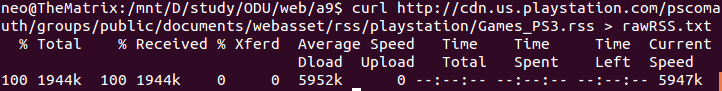
\includegraphics[width=7in]{p1.png}
\end{figure}

\end{homeworkProblem}

%----------------------------------------------------------------------------------------
%	PROBLEM 2
%----------------------------------------------------------------------------------------
\begin{homeworkProblem}
Manually classify the first 50 entries, and then classify (using
the fisher classifier) the remaining 50 entries. \\
\\
Create a table with the title, predicted category, actual category,
and cprob() and fisherprob() for the actual category.\\
\centerline{SOLUTION}
To get cprob and fisherprob, we must have actual category of every entries.\\
In order to get enough words for classifying, here we combined title with summary together as training data.\\
The script will first come out a predicted category, then ask user to input its actual category.\\
For first 50 entries, the user input will then used as training data. For the rest of entries, the user input will be just stored for performance measure in problem 3.\\
Note that raw page contains html tags, we have to remove them at first.\cite{html}
\pythonscript{p2}{Python script for classify entries}


\footnotesize
\begin{longtable}{|l|l|l|l|l|}
\caption{Game Category Table}\\
\hline
\textbf{Title} & \textbf{Predicted} & \textbf{Actual} & \textbf{cprob} & \textbf{fisherprob} \\ \hline
BlazBlue: Chrono Phantasma & fighting & fighting & 0.000000 & 0.999261 \\ \hline
MLB® 14 The Show™ & sports & sports & 0.000000 & 0.632189 \\ \hline
Ragnarok Odyssey ACE & rpg & rpg & 0.000000 & 0.992042 \\ \hline
Batman™: Arkham Origins Blackgate - Deluxe Edition & arpg & arpg & 0.000000 & 0.988878 \\ \hline
Jimmie Johnson's Anything With An Engine™ & fighting & racing & 0.000000 & 0.716525 \\ \hline
TRINITY: Souls of Zill O'll™ & fighting & rpg & 0.000000 & 0.747023 \\ \hline
FEZ & rpg & platform & 0.000000 & 0.750000 \\ \hline
Dynasty Warriors 8: Xtreme Legends & rpg & action & 0.000000 & 0.900965 \\ \hline
Deception IV: Blood Ties & rpg & arpg & 0.000000 & 0.837869 \\ \hline
Cabela's® Big Game Hunter® Pro Hunts & sports & fps & 0.000000 & 0.901288 \\ \hline
TNN® Motorsports HardCore TR™ & fighting & racing & 0.000000 & 0.923191 \\ \hline
Call of Duty®: Ghosts Gold Edition & fighting & fps & 0.000000 & 0.954866 \\ \hline
The Witch and the Hundred Knight™ & fighting & arpg & 0.000000 & 0.454264 \\ \hline
WARRIORS: Legends of Troy™ & fighting & action & 0.000000 & 0.821084 \\ \hline
METAL GEAR SOLID V: Ground Zeroes & fighting & action & 0.000000 & 0.922060 \\ \hline
FINAL FANTASY® X/X-2 HD Remaster & action & rpg & 0.000000 & 0.238850 \\ \hline
YAIBA™: Ninja Gaiden Z & action & action & 0.000000 & 0.864301 \\ \hline
LUFTRAUSERS & action & action & 0.000000 & 0.750000 \\ \hline
Atelier Escha and Logy $\sim$Alchemists of the Dusk Sky$\sim$ & action & rpg & 0.000000 & 0.871188 \\ \hline
Dark Souls™ II & action & arpg & 0.000000 & 0.921179 \\ \hline
Vessel & action & platform & 0.000000 & 0.750000 \\ \hline
South Park™: The Stick of Truth™ & rpg & rpg & 0.000000 & 0.489661 \\ \hline
Master Reboot & action & action & 0.000000 & 0.335016 \\ \hline
NASCAR '14 & action & racing & 0.000000 & 0.833333 \\ \hline
Growlanser®: Heritage of War & action & rpg & 0.000000 & 0.943089 \\ \hline
Tales of Symphonia™ & action & rpg & 0.000000 & 0.860586 \\ \hline
Tales of Symphonia™ Dawn of the New World™ & rpg & rpg & 0.000000 & 0.332998 \\ \hline
Herc's Adventures® & racing & rpg & 0.000000 & 0.918752 \\ \hline
Castlevania: Lords of Shadow 2 & rpg & action & 0.000000 & 0.943089 \\ \hline
THIEF & action & action & 0.000000 & 0.750000 \\ \hline
Magus & action & arpg & 0.000000 & 0.750000 \\ \hline
PAC-MAN MUSEUM™ & action & action & 0.000000 & 0.764077 \\ \hline
Assassin’s Creed® Freedom Cry & action & arpg & 0.000000 & 0.620316 \\ \hline
Neo Contra & rpg & platform & 0.000000 & 0.886142 \\ \hline
Forest Legends: The Call of Love & rpg & platform & 0.000000 & 0.405915 \\ \hline
Mr. Driller & racing & platform & 0.000000 & 0.750000 \\ \hline
Tomba! 2 & rpg & platform & 0.000000 & 0.750000 \\ \hline
Strider® & action & platform & 0.000000 & 0.750000 \\ \hline
Earth Defense Force 2025 & action & action & 0.000000 & 0.852366 \\ \hline
Pac-Man World™ 20th Anniversary & rpg & platform & 0.000000 & 0.712452 \\ \hline
LIGHTNING RETURNS™: FINAL FANTASY® XIII & action & arpg & 0.000000 & 0.473854 \\ \hline
Wolf Fang & action & platform & 0.000000 & 0.560622 \\ \hline
Far Cry® Classic & action & fps & 0.000000 & 0.632608 \\ \hline
Zombeer® & action & action & 0.000000 & 0.750000 \\ \hline
Blowout & racing & platform & 0.000000 & 0.750000 \\ \hline
Dustforce & action & platform & 0.000000 & 0.750000 \\ \hline
Truck Racer & action & racing & 0.000000 & 0.918752 \\ \hline
Trapt & platform & action & 0.000000 & 0.750000 \\ \hline
Adam's Venture: Chronicles & rpg & rpg & 0.000000 & 0.968161 \\ \hline
Gex: Enter the Gecko & racing & platform & 0.000000 & 0.393812 \\ \hline
DRAGON BALL Z: BATTLE OF Z & action & fighting & 0.000000 & 0.695500 \\ \hline
Cyber Sled™ & racing & action & 0.000000 & 0.742811 \\ \hline
THE FIREMEN 2: PETE and DANNY & rpg & arpg & 0.000000 & 0.411317 \\ \hline
Mark Davis Pro Bass Challenge™ & action & sports & 0.000000 & 0.466829 \\ \hline
Lucifer Ring & action & action & 0.000000 & 0.596574 \\ \hline
Assassin’s Creed® Liberation HD & action & action & 0.000000 & 0.257590 \\ \hline
The Raven - Legacy of a Master Thief & action & platform & 0.000000 & 0.060845 \\ \hline
Twisted Lands: Shadow Town & action & rpg & 0.000000 & 0.368775 \\ \hline
Tiny Brains & rpg & rpg & 0.000000 & 0.596574 \\ \hline
Dragon Fantasy Book I and II Bundle & rpg & rpg & 0.000000 & 0.339384 \\ \hline
The Walking Dead: Season Two & action & rpg & 0.000000 & 0.226454 \\ \hline
flOw & action & rpg & 0.000000 & 0.166667 \\ \hline
Mutant Mudds Deluxe & action & action & 0.000000 & 0.384503 \\ \hline
Aabs Animals & platform & rpg & 0.000000 & 0.596574 \\ \hline
Toki Tori & action & platform & 0.000000 & 0.596574 \\ \hline
The Walking Dead: Season 2 - Ep.1, All That Remains & action & rpg & 0.000000 & 0.111491 \\ \hline
Minecraft & action & arpg & 0.000000 & 0.500000 \\ \hline
Strength Of The Sword 3 & action & action & 0.000000 & 0.197681 \\ \hline
Doki-Doki Universe™ & rpg & platform & 0.000000 & 0.290409 \\ \hline
Gran Turismo® 6 & action & racing & 0.000000 & 0.384930 \\ \hline
Doki-Doki Universe™ & rpg & platform & 0.000000 & 0.290409 \\ \hline
Doki-Doki Universe™ & rpg & platform & 0.000000 & 0.290409 \\ \hline
Oddworld: Abe Boxx & platform & platform & 0.000000 & 0.655185 \\ \hline
Painkiller - Hell and Damnation & action & fps & 0.000000 & 0.655185 \\ \hline
Super Motherload & action & action & 0.000000 & 0.596574 \\ \hline
Saint Seiya: Brave Soldiers + Aries Shion & action & action & 0.000000 & 0.591461 \\ \hline
Young Justice: Legacy & action & action & 0.000000 & 0.104574 \\ \hline
Arcania - The Complete Tale & action & rpg & 0.000000 & 0.236300 \\ \hline
CONTRAST™ & rpg & rpg & 0.000000 & 0.500000 \\ \hline
Need for Speed™ Rivals & action & racing & 0.000000 & 0.181262 \\ \hline
ADVENTURE TIME: EXPLORE THE DUNGEON BECAUSE I DON'T KNOW! & action & action & 0.000000 & 0.216729 \\ \hline
AquaPazza™ & action & fighting & 0.000000 & 0.500000 \\ \hline
SOULCALIBUR®II HD ONLINE & action & fighting & 0.000000 & 0.199787 \\ \hline
Farming Simulator & action & rpg & 0.000000 & 0.596574 \\ \hline
Air Conflicts: Vietnam & action & action & 0.000000 & 0.655185 \\ \hline
Stick It To The Man & action & action & 0.000000 & 0.107770 \\ \hline
Blood Knights & action & rpg & 0.000000 & 0.235787 \\ \hline
Wonderbook™: Walking with Dinosaurs & action & platform & 0.000000 & 0.376061 \\ \hline
Wonderbook™: Book of Potions & rpg & platform & 0.000000 & 0.476013 \\ \hline
Wonderbook™: Diggs Nightcrawler™ & action & platform & 0.000000 & 0.655185 \\ \hline
XCOM®: Enemy Within & action & action & 0.000000 & 0.340747 \\ \hline
Injustice: Gods Among Us Ultimate Edition & action & fighting & 0.000000 & 0.056800 \\ \hline
Ratchet and Clank: Into the Nexus™ & action & action & 0.000000 & 0.193413 \\ \hline
Call of Duty®: Ghosts & fps & fps & 0.000000 & 0.931765 \\ \hline
Call of Duty®: Ghosts Digital Hardened Edition & action & fps & 0.000000 & 0.829427 \\ \hline
How to Survive & action & action & 0.000000 & 0.742811 \\ \hline
The Adventures of Cookie and Cream & action & action & 0.000000 & 0.236300 \\ \hline
A-men 2 & action & platform & 0.000000 & 0.166667 \\ \hline
The Guided Fate Paradox & action & rpg & 0.000000 & 0.411317 \\ \hline
Ben 10 Omniverse™ 2 & action & action & 0.000000 & 0.596574 \\ \hline
\end{longtable}
\normalsize

\end{homeworkProblem}
%----------------------------------------------------------------------------------------
%	PROBLEM 3
%----------------------------------------------------------------------------------------
\begin{homeworkProblem}
Assess the performance of your classifier in each of your
categories by computing precision, recall, and F-measure.  \\
\centerline{SOLUTION}
First we have to get numbers of true positive, false positive and false negative in each category.\\
Here we use python to iterate through each record above compare the predicted category and actual category, then sum them in a table.\\
Then, use formula provided in the slide to get precision, recall and f-measure.
\pythonscript{p3}{Python code to assess the performance}
\begin{table}[h]
\centering
\caption{Statistics about TP,FP and FN for each category}
\begin{tabular}{|l|l|l|l|}
\hline
\textbf{Category} & \textbf{TP} & \textbf{FP} & \textbf{FN} \\ \hline
platform & 1 & 2 & 21 \\ \hline
fps & 1 & 0 & 5 \\ \hline
rpg & 7 & 13 & 15 \\ \hline
action & 22 & 38 & 6 \\ \hline
arpg & 1 & 0 & 8 \\ \hline
racing & 0 & 5 & 6 \\ \hline
fighting & 1 & 7 & 4 \\ \hline
sports & 1 & 1 & 1 \\ \hline
\end{tabular}
\end{table}

\begin{table}[h]
\centering
\caption{Performance}
\begin{tabular}{|l|l|l|l|}
\hline
\textbf{Category} & \textbf{Precision} & \textbf{Recall} & \textbf{F-measure} \\ \hline
platform          & 0.333333           & 0.045455        & 0.080000           \\ \hline
fps               & 1.000000           & 0.166667        & 0.285714           \\ \hline
rpg               & 0.350000           & 0.318182        & 0.333333           \\ \hline
action            & 0.366667           & 0.785714        & 0.500000           \\ \hline
arpg              & 1.000000           & 0.111111        & 0.200000           \\ \hline
racing            & 0.000000           & 0.000000        & 0.000000           \\ \hline
fighting          & 0.125000           & 0.200000        & 0.153846           \\ \hline
sports            & 0.500000           & 0.500000        & 0.500000           \\ \hline
\end{tabular}
\end{table}
*A nice online tool for converting raw table file to latex is recommended here:\\
\url{http://www.tablesgenerator.com}
\end{homeworkProblem}

\bibliographystyle{plain}
\bibliography{ref}
\end{document}